\section{Energy Modeling}
\label{sec:EnergyModeling}
Consider that the two seemingly best performing LPWAN technologies, LoRa and NB-IoT, are possible choices for our Elephant Tracking Application. We will now compare the energy consumption of these two technologies. 

As a constant, we will need to fix the Infrared Sensor that we will use in our application. For the purposes of this report, we will assume there is direct hardware compatability with the sensor and the LPWAN technology, and that we have done a control trial of using a smaller IR Sensor for detecting motion of the elephants at that specific range setting. 

The IR sensor we will be using is the \textit{GUMP's grocery HC-SR501 Infrared PIR Motion Sensor}\cite{GumpSensor}. This sensor has a range of 7 meters, and a power consumption of 60 $\mu$A, and since our operation will most likely be at the top end of its operational limit (farther to $7$ meters), we will assume that the device is operating at $20V$. Roughly speaking, we use this sensor as it is small and inconspicuous, and can be placed in the forest without being noticed by the elephants. That being said, the efficacy of the sensor is still in question, especially in a dense forest environment.\\
% \begin{figure}[!h]
    \centering
    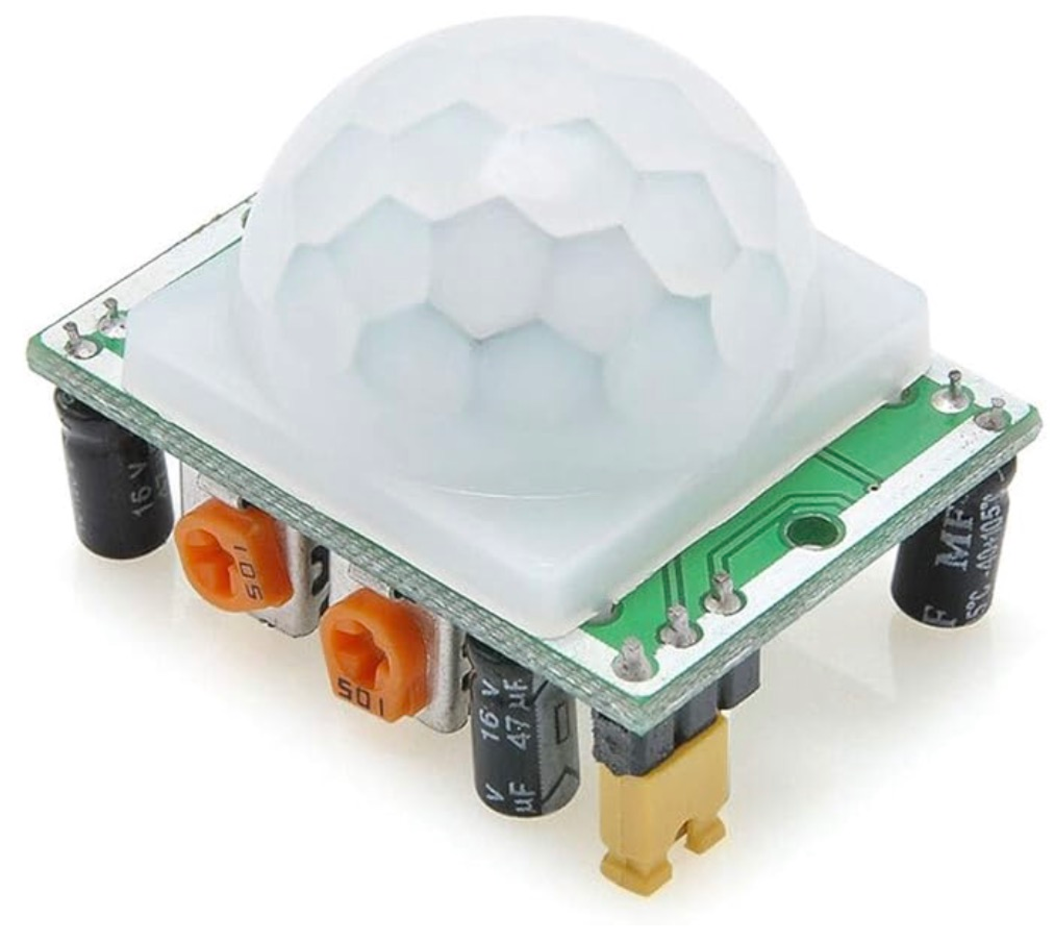
\includegraphics[width=0.6\columnwidth]{figures/Gump.pdf}
    \caption{GUMP HC-SR501 Infrared PIR Motion Sensor.}
    \label{fig:gump}
\end{figure}
\subsection{LoRa}
\label{sec:LoRa}
Our Application is based in Kerala $ + $ Tamil Nadu in India, so our LoRA specifications are different than the conventional US guidelines. In particular, in India we are able to use any Spreading Factor (SF) from SF7 to SF12, at 125 kHz bandwidth. This is because the Indian government has allocated the 865-867 MHz band for LoRaWAN use, which is different from the US guidelines. Another important thing is that according to \cite{loraGuidelines}, \textbf{there is no dwell or duty-cycle limitation on LoRA transmission}, according to Section 2.10.3 (IN865-867 Data Rate and End Device Output Power Encoding).
\todo{Insert Figure of Table here}


Table \ref{tab:lora_power} has some truncated findings that are also found in screenshots (linked in appendix) from the Lora Guidelines. For our purposes, since we are using a Lora Module (I assume that we are using the SX1262 for transmit), and we will be comparing the power consumption of the device in both DC-DC and LDO mode. The LDO mode is more power hungry, and the DC-DC mode is more efficient. 

Consider the operating modes that we defined earlier: 
\begin{itemize}
    \item Steady State Sensing
    \item Event-Driven Update
    \item Emergency Mode
\end{itemize}
\subsubsection{Turning Off and On}
Since our time interval is so large, turning off the radio and then turning on will be marginal relative to the power consumption of the device. This is because either we will sleep for a long time, or we will be receiving for a long time, and the power consumption relative to the major operations of the device is in the order of nanoAmps versus Milliamps (nearly a factor of $10^6$). Susbequently, the datasheet provides the power consumption of the device in Sleep, but not necessarily the power consumption it takes to turn on the device $\rightarrow$ for the purposes of this report, we will assume that the power consumption of turning on the device is negligible (as a couple milliseconds relative to the 5 minute interval is not significant). 
In Steady State, the device will be in Standby Mode for 5 minutes, wake up and second a transmission, and then go back to Standby/standby. The power consumption for the standby duration is given by $800 nA \times 3.3 V * 300 s = 792\mu J$. This is with the crystal clock setting (XOSC) on. Then in Transmit this varies based on the power setting, let's see which mode is best for our application. 

Now the possible configurations we have for LoRA are 
$SF7, SF8, SF9, SF10, SF11, SF12$ at $125 kHz$ bandwidth. Then we can choose the power setting for the device, which can be $+14 dBm, +17 dBm, +20 dBm, +22 dBm$, as well as which mode we want to be in for hardware state (DC-DC or LDO).

For Steady State Sensing, we will sense for 1 second every 5 minutes, and then transmit accordingly based on our Spreading Factor prior to going back to standby. 

In general we have the formula $$E_{tx} = (\frac{P_{size}}{R} * I_{tx} * V_{opt}) * T_{tx} + E_{rest}$$, where $P_{size}$ is the packet size, $R$ is the data rate, and the other terms are the current, the operating Voltage, and the standby Energy. 

The Data rate will be dependent on the Spreading Factor, and the Current for Transmission will be dependent on the power setting.
\subsection{Steady State Transmission}
In essence, Table \ref{tab:lora_power_revised} contains simulated results of running the LoRa device under a Steady State configuration for 24 hours. The results are based on the power consumption of the device in different modes. Operating at SF7 with the lowest power setting of +14 dBm, the device consumes 1.229 mJ of energy over 24 hours, and this makes sense as the "chirps" are shorter and so messages can be transmitted faster. Intuitively, the higher the spreading factor, the more energy is consumed due to the longer chirps. At the highest end, SF12 with +22 dBm with a PA Target of +22 dBm, the device consumes 57.647 mJ of energy over 24 hours. This is a significant amount of energy, and it is clear that the device is not optimized for this setting. A configuration that strikes a sweet balance between energy consumption and data rate is SF7 with a +22 target with a Transmit Power of 22 dBm. This is the highest setting for the device, but by transmitting at a higher power, we still get a good data rate and a decent energy consumption of only 2.852 mJ over 24 hours, while still taking advantage of the LoRA's long range capabilities.

\subsection{Event-Driven Update}
In the cases where we do an update based on an event, ideally this is akin to a \textbf{Firmware Update} or a \textbf{Critical Event}. In this case, this is a downlink event where we will download a new patch, of 10 MB in size. Depending on our configuration, we can either use the DC-DC mode or the LDO mode. The DC-DC mode is more efficient, but the LDO mode is more power hungry.


It seems configuring the device to be in DC-DC mode is the best option for our firmware updates, as the power consumption is lower than in the LDO Mode. While we care about data integrity, the marginal optimization that LDO mode provides is not worth around 4 times the power consumption. Table \ref{tab:lora_rx} shows the power consumption of the device in the receive mode, and it is clear that the DC-DC mode is the best option for our application.

\subsection{Emergency Mode}

When the device is in Emergency Mode, we will be transmitting at the highest power setting, and we will be transmitting at the highest spreading factor. This is because we want to maximize the integrity of the device, and we want to ensure that the message is received. In this case, we will be transmitting at SF12, with a power setting of +22 dBm. This is the highest power setting for the device, and it is clear that the device is not optimized for this setting. The device consumes 1.638 J of energy over 24 hours, and this is a significant amount of energy. This is not a good setting for the device, and it is clear that the device is not optimized for this setting. We still aim to strike a good balance between power and data integrity, and we can still transmit at SF 12 with a +22 dBm power setting, but we will need to be more careful with our power consumption. A concern that is often brought up is that SF12 could cause an overlap in the chirps. This is a valid concern, but with our current packet structure of 16 bytes, we can still transmit at SF12 as the $TX$ duration is $\frac{16 * 8}{250} = 0.512 s$, which is less than the 10 second intermission between transmission.
\begin{figure*}[h!]
    \centering
    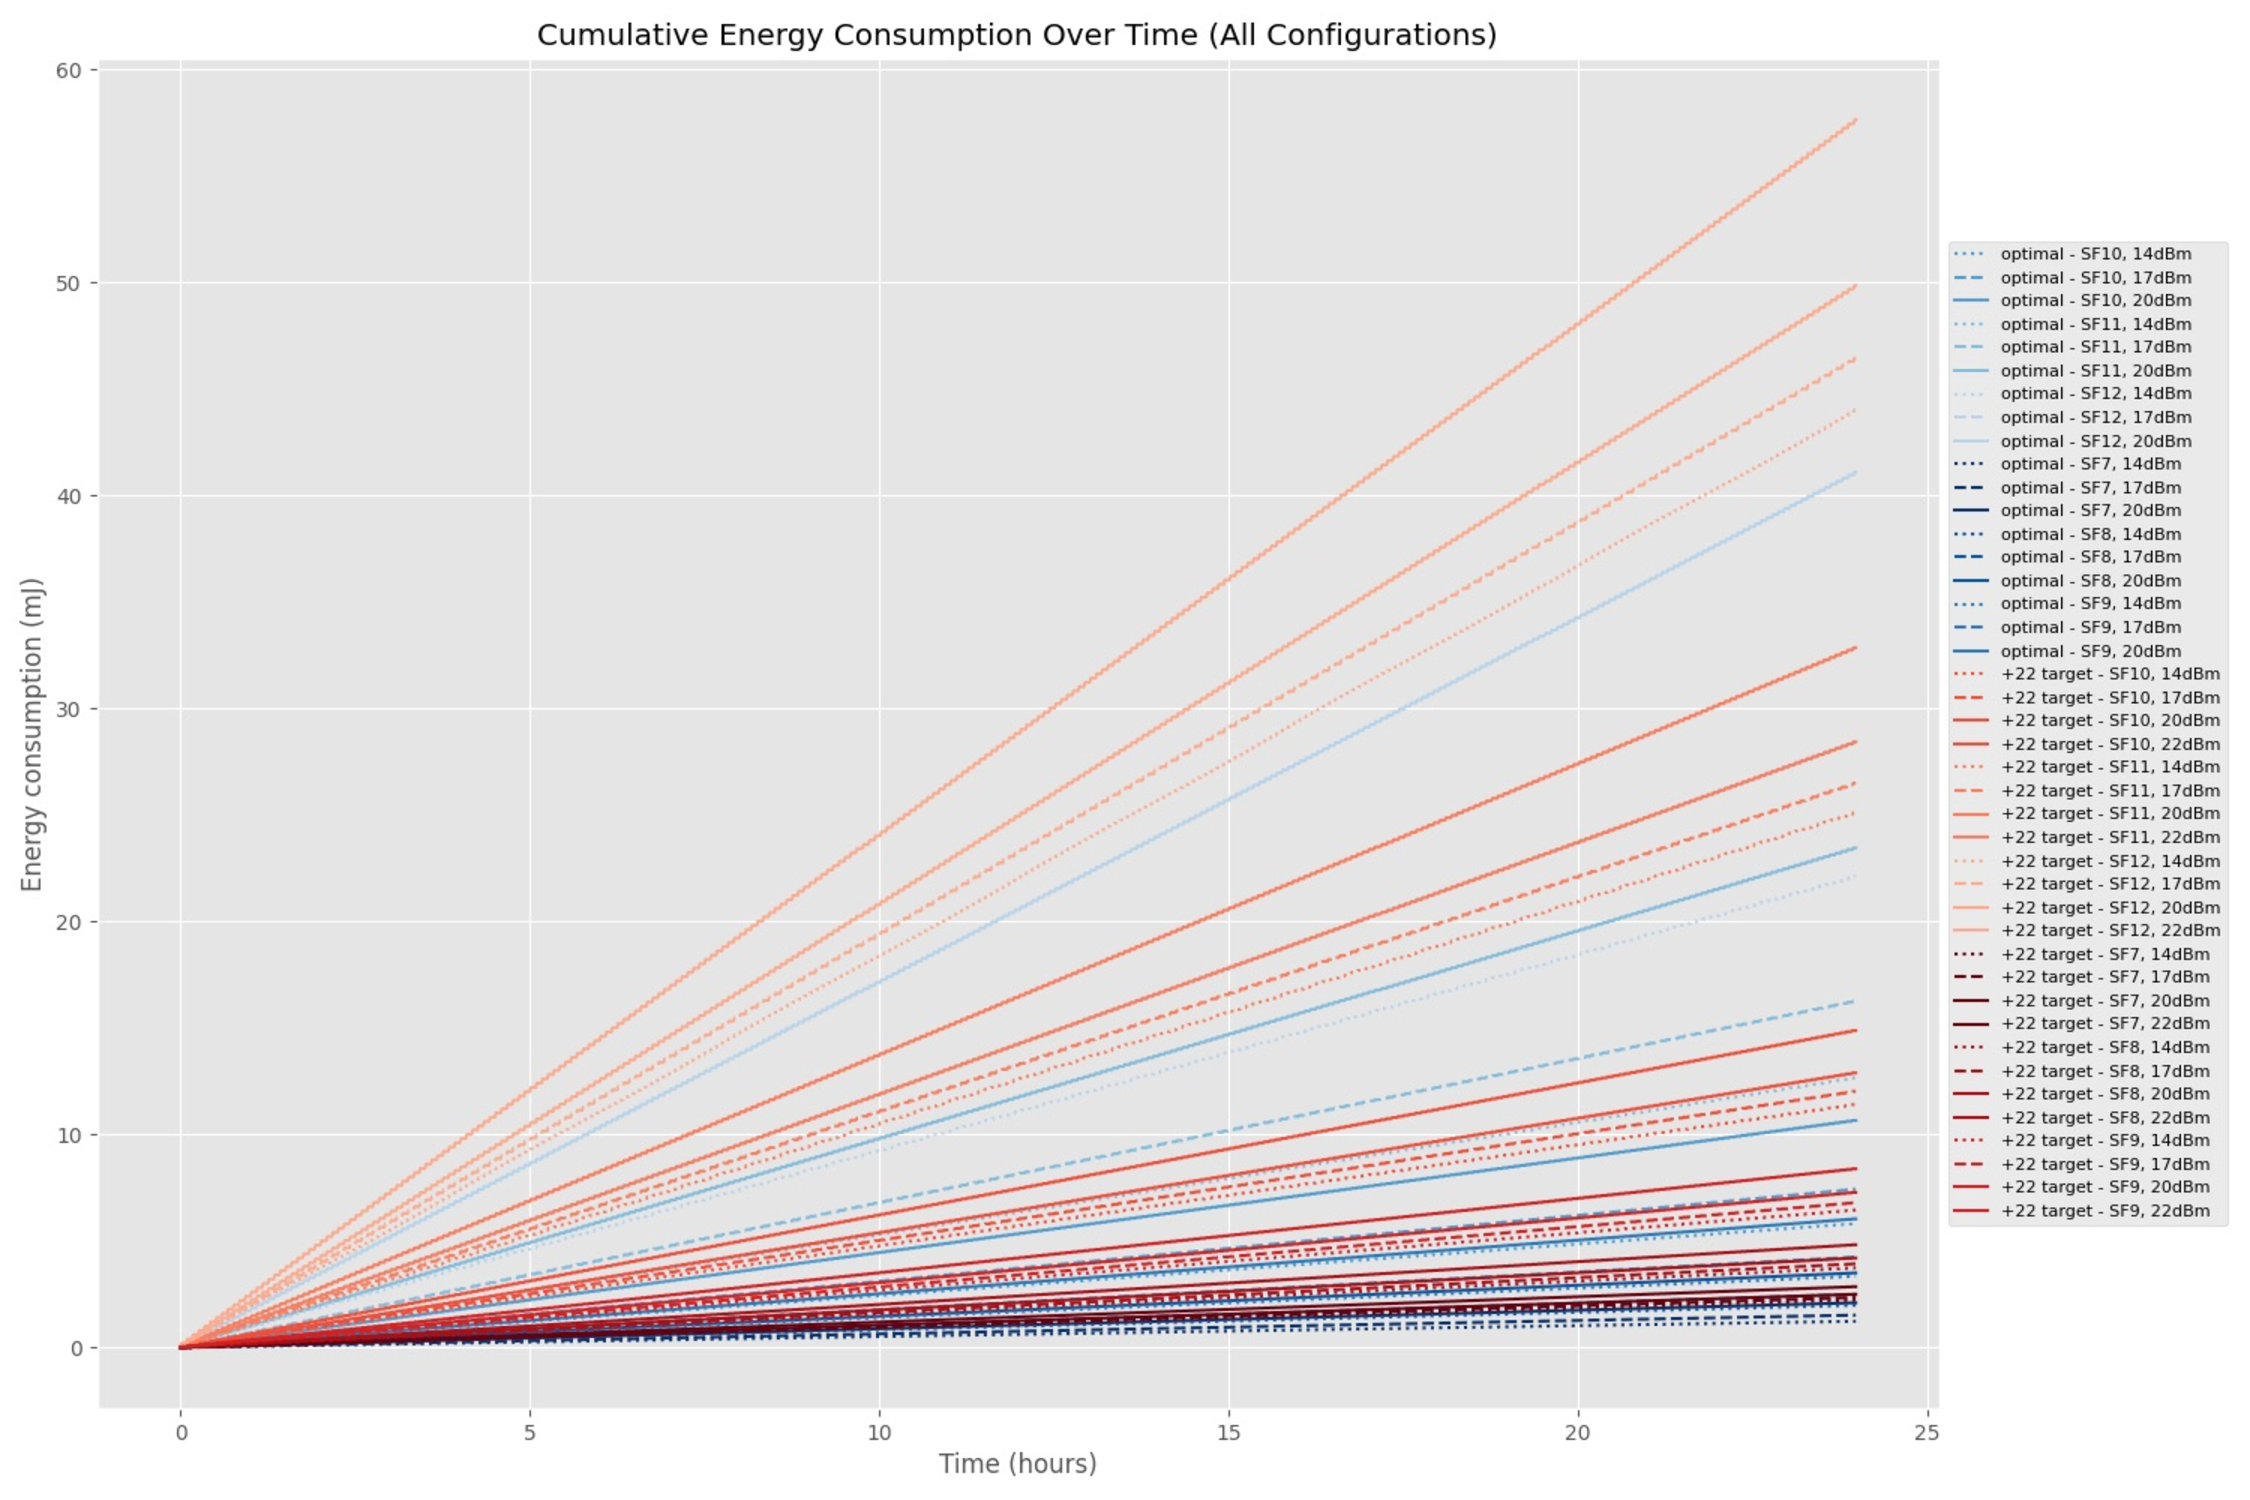
\includegraphics[width=\textwidth]{figures/loraTXSS.pdf}
    \caption{LoRa Device Power Consumption in Transmit Modes}
    \label{fig:loraTXSS}
\end{figure*}
\begin{figure}[h!]
    \centering
    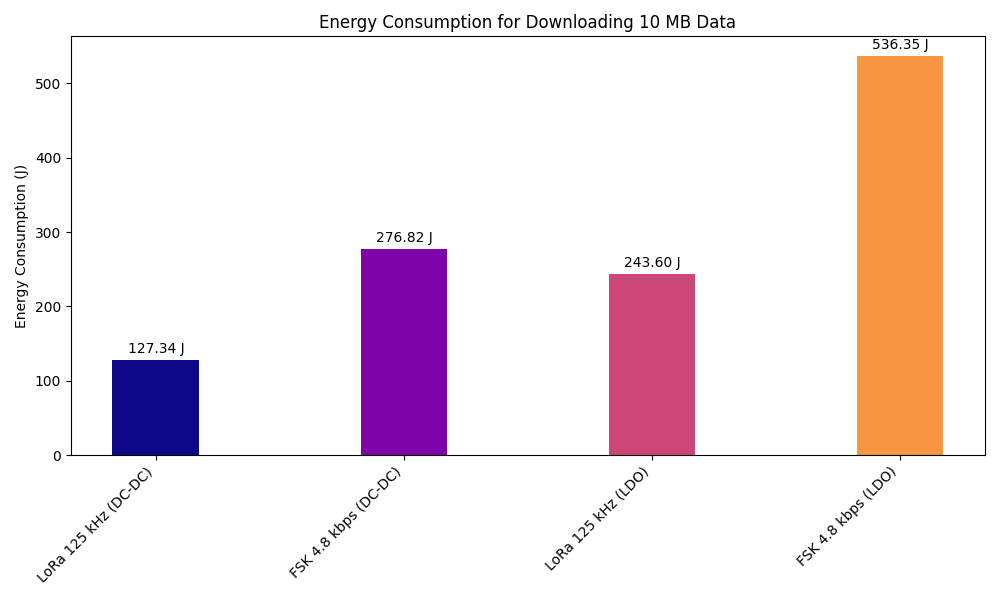
\includegraphics[width=\columnwidth]{figures/loraRx.png}
    \caption{LoRa Device Power Consumption in Receiving Firmware Update}
    \label{fig:loraRx}
    
\end{figure}
\begin{figure}[h!]
    \centering
    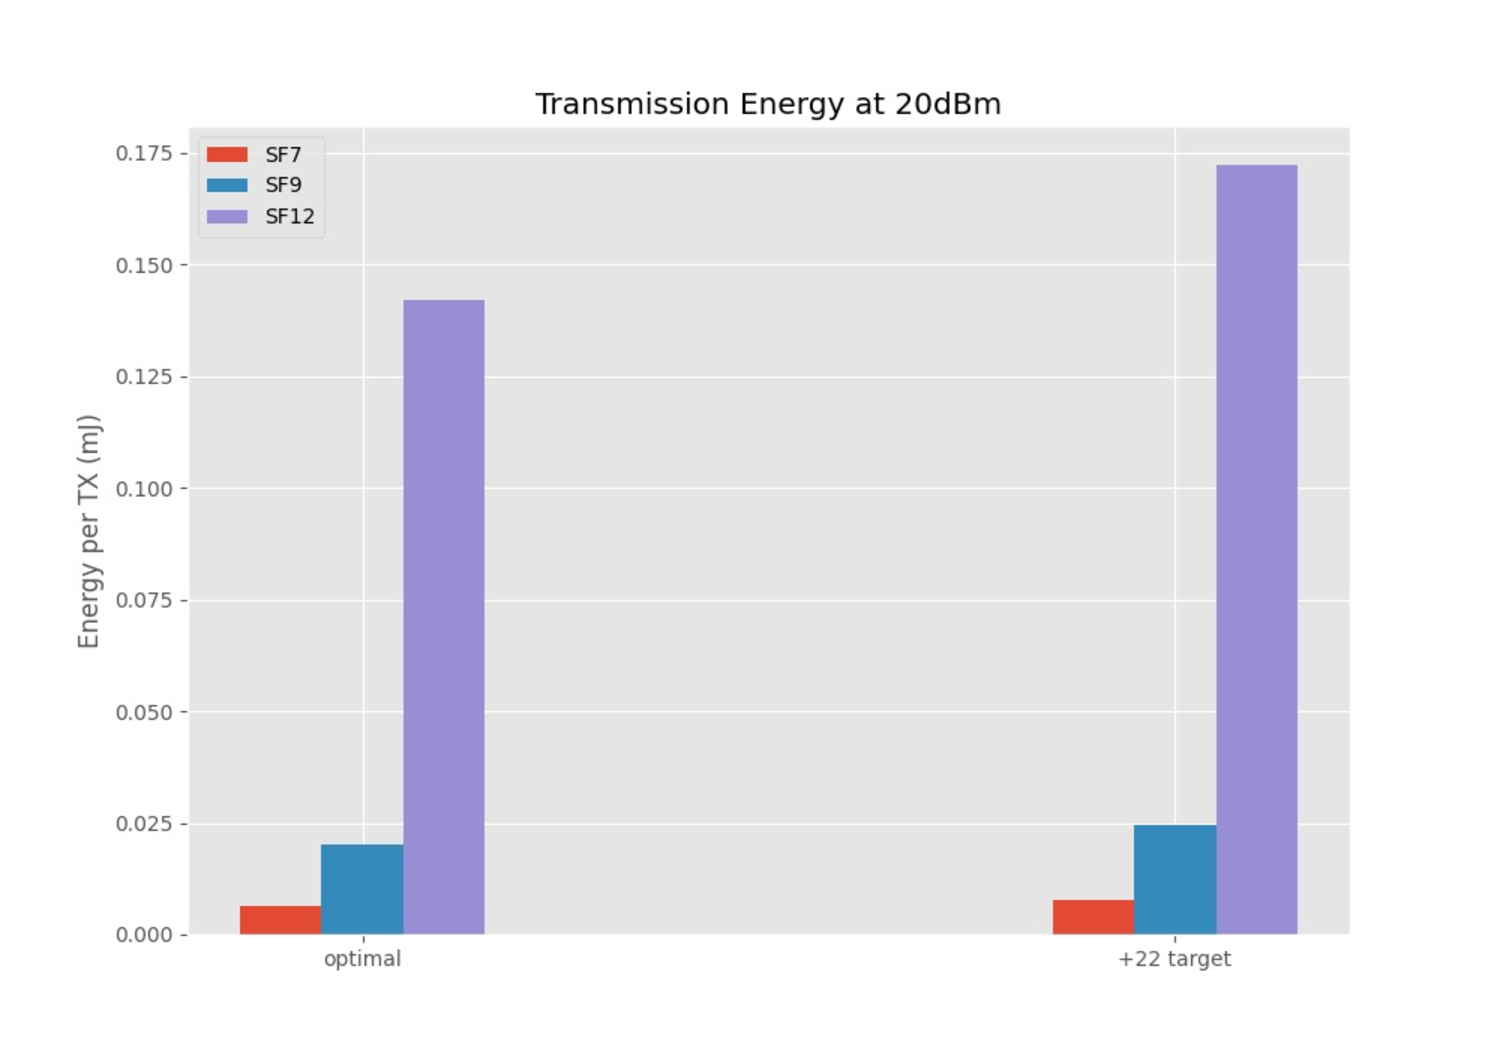
\includegraphics[width=\columnwidth]{figures/loratx20dbmbar.pdf}
    \caption{LoRa Device Power Consumption transmitting at +20 dBm}
    \label{fig:loratx20dbmbar}
\end{figure}

\subsection{NB-IoT}
\label{sec:NB-IoT}

Our Application can rely on the already existing 4G Infrastructure that already covers the entirety of continental India. That being said, power wise we don't have to deal with the complexities of changing a Spreading Factor Unlike LoRA, but we will have to tune some parameters to deal with our three different operating modes. 

The NB-IoT device will be in a similar configuration to the LoRA device, but the power consumption will be different. The device will be in Standby Mode for 5 minutes, wake up and send a transmission, and then go back to Standby/standby. The power consumption for this module is given by the same formula, but the current and voltage will be different. For brevity, \textbf{We will fix the module to the Sara R510S} for power consumption reasons (the initial deployment cost/cost of goods does not outweigh the module being performant for the entire year long pilot.)

Using the data sheet in \cite{nbPower}, there are many configurations for which we can configure the chip. Due to Discontinuous Reception (DRX), and Extended Discontinuous Reception (eDRX), we can model the power consumption of the device using different intervals. This plays to the strength of NB-IOT, where sleeping for a long time is beneficial, as this means less wake ups to sync with the central tower, and less power consumption overall. Also, while the device is operating, the typical operating voltage is $3.8V$ but this value ranges from $3.3 \sim 4.4$ V.

The main tradeoff with the NB-IOT approach is that while sleep mode is around the same as LORA, transmission is very high (around $2\sim3$ the magnitude to transfer at the same power strength as LoRA). But this is is a high level artifact of the technology, that can only be absorobed in our implementation due to current adoption standards of LoRA in India (and the ubiquitous nature of 4G and 5G in the region).






